\label{chap:analise}
Conforme identificado no capítulo \ref{chap:introducao}, em posse
dos dados, devemos classificá-los de forma a identificar os diferentes
segmentos de mercado na população, verificar para quais desses segmentos
o produto é mais interessante e direcionar a comunicação e criar a
campanha de marketing de forma a atingir essa parte da população.

A ferramenta de análise utilizada para resolução desse problema será
a Análise de Cluster, também conhecida como análise de conglomerados.

A análise de cluster é uma técnica de análise multivariada cujo principal
objetivo é reunir pontos de dados baseando-se nas características
individuais de cada um. Ou seja, ele classifica cada elemento segundo
aquilo que cada um tem de similar em relação a outros pertencentes
a um determinado grupo, considerando um critério de seleção predeterminado.

O resultado da Análise de Cluster deve exibir um alto grau de homogeneidade
interna (dentro do cluster) e alto grau de heterogeneidade externa
(entre os diferentes clusters) conforme demonstrado na figura \ref{fig:clustering}.

\begin{figure}
\begin{centering}
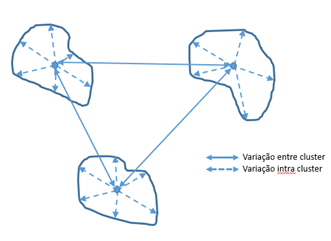
\includegraphics[width=0.65\textwidth]{Imagens/clustering}
\par\end{centering}

\caption{\label{fig:clustering}Heterogeneidade e homogeneidade}
\end{figure}


Esse tipo de análise é utilizada em diferentes campos de estudo, como
psicologia, biologia, marketing, engenharia, administração e contabilidade.
Entretanto em todos esses campos a análise tem um objetivo comum.
Classificar os elementos de acordo com os relacionamentos naturais.

Existem diferentes maneiras e técnicas de se aplicar esse tipo de
análise, em nosso caso será utilizado o método de Ward, que é um método
no qual a soma dos quadrados dos desvios de cara elemento em relação
a cada conglomerado é minimizada. Esse método tem uma tendência a
combinar grupos com um menor número de observações e produz grupos
com aproximadamente o mesmo número de elementos.

Por fim, ao final da análise deve-se interpretar os resultados, o
que envolve o exame de cada grupo levando em conta o conjunto de variáveis
eleitas para atribuir uma identificação que descreva adequadamente
a natureza dos grupos.

No caso estudado a análise de cluster mostra-se especialmente útil
pois ela classifica os elementos em diferentes segmentos de mercado
e auxilia na escolha de qual protótipo seria mais indicado a cada
grupo, bem como indicaria qual o tipo de comunicação deveria ser feita
a cada grupo após escolhido o protótipo.

\begin{figure}
\begin{centering}
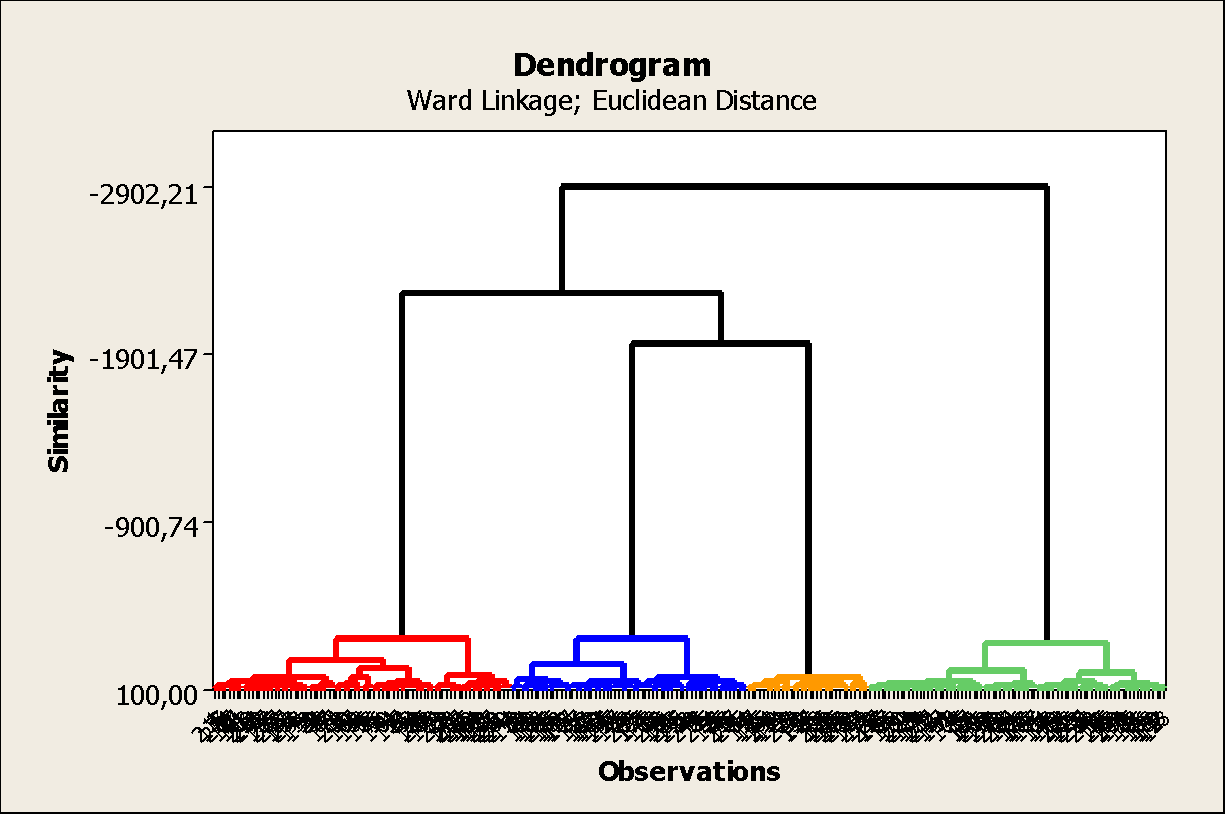
\includegraphics[width=0.85\textwidth]{Imagens/dendogram}
\par\end{centering}

\caption{\label{fig:dendogram}O Dendograma por método de Ward tomados \emph{Imagem,
Utilitário e Preço}.}
\end{figure}


\begin{table}
\begin{centering}
\begin{tabular}{c|c|c|c|c|c}
\hline 
Variável & Cluster 1 & Cluster 2 & Cluster 3 & Cluster 4 & Centróide\tabularnewline
\hline 
Imagem & 2,35 & 3,04 & 0,95 & 0,62 & 2,00\tabularnewline
\hline 
Utilitário & 2,95 & 1,57 & 0,99 & 3,47 & 2,10\tabularnewline
\hline 
Preço & 2,89 & 0,98 & 2,36 & 0,54 & 1,86\tabularnewline
\hline 
\end{tabular}
\par\end{centering}

\caption{\label{tab:centroids-ward}Centróides de clustering obtidos por método
de Ward}
\end{table}


O dendograma apresentado na figura \ref{fig:dendogram} e na tabela
\ref{tab:centroids-ward} denotam a relação entre \emph{Imagem, Preço,
Utilitário }e\emph{ Cluster }que é usada como base na abordagem de
\emph{Persona }neste capítulo. Na tabela, observa-se uma atração do
cluster 1 para \emph{Imagem}, \emph{Utilitário} e \emph{Preço}. Do
cluster 2 para \emph{Imagem}, do 3 para \emph{Preço} e do 4 para \emph{Utilitário}.

